\documentclass[times, utf8, diplomski]{fer}
\usepackage{booktabs}
\usepackage{listings}
\usepackage{amsthm}
\usepackage{algorithmic}
\usepackage{algorithm}

\newtheorem{wirerule}{Rule}
\newtheorem{wiredef}{Definition}

\begin{document}


\thesisnumber{222}

\title{Methods for specification and automatic recognition of network protocols}

\author{Dražen Popović}

\maketitle

\izvornik

\zahvala{
I wish to thank my amazing family for making this dream come true. Thanks to
my friends from the 9th for being there and helping me. Special thanks to my
mentor Doc.dr.sc Domagoj Jakobović for getting me out of messy situations and for
putting up with me.

\emph{So Long, and Thanks for All the Fish! :)}
}

\tableofcontents

\chapter{Introduction}
The thesis starts with giving an overview on network protocol theory including
protocol design, specification and implementation. This provides the appropriate
terminology and a knowledge framework for developing a network protocol specification
language, called \emph{Wire}. A custom protocol is developed to demonstrate Wire, thus
showing its motivation, purpose and inner workings. Detailed descriptions are 
provided on making of the Wire compiler including language analysis and code generation.
The second part of this thesis analyses the task of automatic recognition of
network protocols. The approach taken for solving this problem is evolutionary
computation technique, more specifically genetic algorithms. By utilizing the 
\emph{Evolutionary Computation Framework}, a network protocol genotype
and corresponding genetic operators are described and implemented.

\chapter{Wire definition language}
Wire is a network protocol definition language derived from \emph{Interface Definition Language} (IDL)\footnote{IDL is a specification language used to describe a software component's interface.}. 
It is used to represent an on the wire representation of a certain network protocol in an intuitive and highly abstract manner. 
The Wire compiler is designed to address the automatic generation of code that handles all of the defined protocol's communications, parsing and construction of packets. 

Coding handlers for network protocols is time consuming and highly error prone. 
One must deal with sanity checks upon packet parsing/construction, integer byte ordering and sizes, various charset encodings, data alignment and padding, error reporting and debugging. 
Furthermore when considering protocol operations, programmers must take into account memory allocation and buffering, timing, various types of operations such as blocking/nonblocking (synchronous/asynchronous) operations.
Programmers take various approaches for tackling coding of network protocol handlers and thus code reusability is low, modularity is weak and uniformity is non-existent (in most cases). 

Wire is intended to provide an intuitive way of defining a protocol that can be situated in \emph{Link}, \emph{Network}, \emph{Transport} or \emph{Application} layer. 
Furthermore the code generated by the compiler fits nicely with the network protocol theory and as such is easy readable. 
The API provided by the generated code library tends to be simple and easy to use, but of course that depends on the protocol definition. 
To that point Wire strives to provide an abstraction to its users from underlying networking technologies (\emph{Berkley sockets}, \emph{WinSock}, \emph{TLI}) and host configurations (byte/bit ordering, register sizes, floating point representations, character encodings).

The initial idea for Wire was to create a definition language in which one would define a protocol, run it trough a compiler and get a program library that would handle that particular network protocol. The protocol at hand is already suppose to have a specification such as \emph{Internet protocol} (IP) or even \emph{Hyper Text Transfer Protocol} (HTTP). 
Thus with a single Wire definition a compiler could generate handlers in multiple languages and/or for various systems and frameworks. 
For example code generation could be extended to generate \emph{Lua} libraries or more specifically \emph{NMAP NSE} libraries which are written in Lua but exist in a more specialized framework. 
Also one could generate dissection methods for \emph{Wireshark}.
The natural extension to the initial idea is to define your own network protocol for whatever purposes. 
This makes Wire a definition language and the underlying encoding algorithms a serialization protocol. 
Similar technologies include \emph{ASN.1}, \emph{JSON}, \emph{XDR}.
Wire conceptually differs from mentioned projects in the fact that these projects weren't designed to provide means to define an already existing protocol.
One can, by using Wire, specify the on the wire representation of a defined network protocol at hand.
\section{Network protocol theory}
What is a protocol? A computer protocol can be defined as a well-defined set of messages (bit patterns or, increasingly today, octet strings) each of which carries a defined meaning (semantics), together with the rules governing when a particular message can be sent. 
However, a protocol rarely stands alone. 
Rather, it is commonly part of a \emph{protocol stack}, in which several separate specifications work together to determine the complete message emitted by a sender, with some parts of that message destined for action by intermediate (switching) nodes, and some parts intended for the remote end system.
In this \emph{layered} protocol model:
\begin{itemize}
  \item One specification determines the form and meaning of the outer part of the message, 
  with a \emph{`hole'} in the middle. It provides a \emph{carrier service} (or just \emph{service}) to convey any material that is placed in this `hole'.
  \item A second specification defines the contents of the `hole', perhaps leaving a further `hole' for another layer of specification, and so on. 
\end{itemize}
\begin{figure}[htb]
\begin{center}
\leavevmode
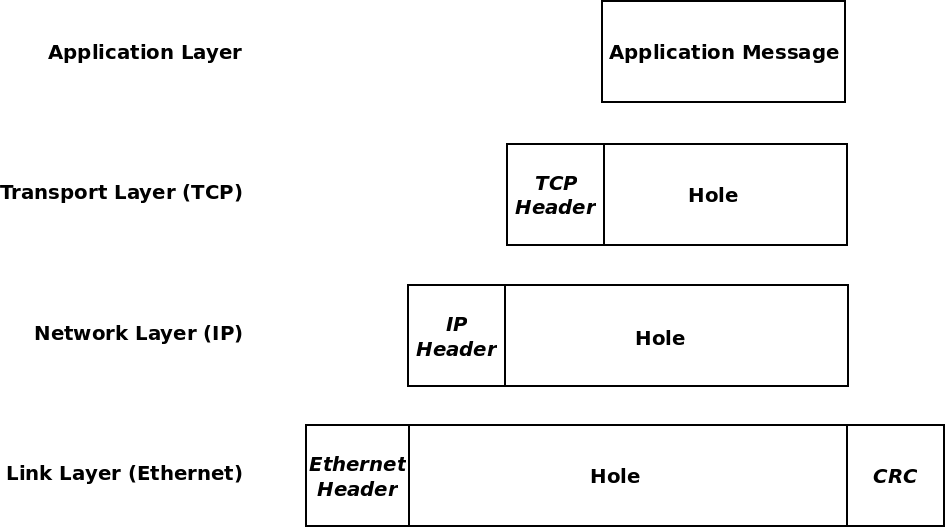
\includegraphics[width=0.8\textwidth]{tcp_ip_model_hole}
\end{center}
\caption{TCP/IP model (`hole')}
\label{fig:tcp_ip_model_hole}
\end{figure}
\ref{fig:tcp_ip_model_hole} illustrates the TCP/IP stack, where real networks provide the basic carrier mechanism, with the IP protocol carried in the `hole' they provide, and with IP acting as a carrier for TCP (or the the less well-known User Datagram Protocol - UDP), forming another protocol layer, and with a (typically for TCP/IP) monolithic application layer - a single specification completing the final `hole'. 
The precise nature of the service provided by a lower layer (lossy, secure, reliable), and of any parameters controlling that service, needs to be known before the next layer up can make appropriate use of that service. We usually refer to each of these individual specification layers as a \emph{protocol}.
Note that in \ref{fig:tcp_ip_model_hole}, the `hole' provided by the IP carrier can contain either a TCP message or a UDP message - two very different protocols with different properties (and themselves providing a further carrier service). Thus one of the advantages of layering is in reusability of the carrier service to support a wide range of higher level protocols, many perhaps that were never thought of when the lower layer protocols were developed. 
When multiple different protocols can occupy a `hole' in the layer below (or provide carrier services for the layer above), this is frequently illustrated by the layering diagram shown in \ref{fig:tcp_ip_layering}
\begin{figure}[htb]
\begin{center}
\leavevmode
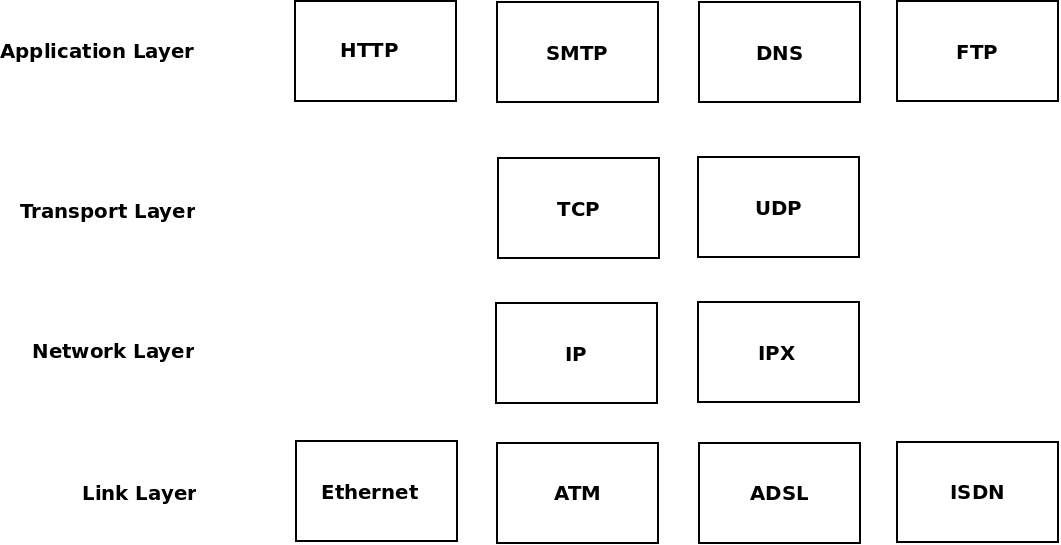
\includegraphics[width=0.8\textwidth]{tcp_ip_layering}
\end{center}
\caption{TCP/IP layering}
\label{fig:tcp_ip_layering}
\end{figure}

\subsection{Layered architecture}
The layering concept is perhaps most commonly associated with the 
\emph{International Standards Organization} (ISO) and \emph{International 
Telecommunications Union} (ITU) architecture or `7-layer model' for \emph{Open 
Systems Interconnection} (OSI) shown in \ref{fig:osi_model}. To reduce their 
design complexity, most networks are organized as a stack of layers or levels, 
each one built upon the one below it. The number of layers, the name of each layer, 
the contents of each layer, and the function of each layer differ from network to network. 
The purpose of each layer is to offer certain services to the higher layers, 
shielding those layers from the details of how the offered services are actually 
implemented. This is know as \emph{encapsulation}. In a sense, each layer is a 
kind of `virtual machine', offering certain services to the layer above it.

\begin{figure}[htb]
\begin{center}
\leavevmode
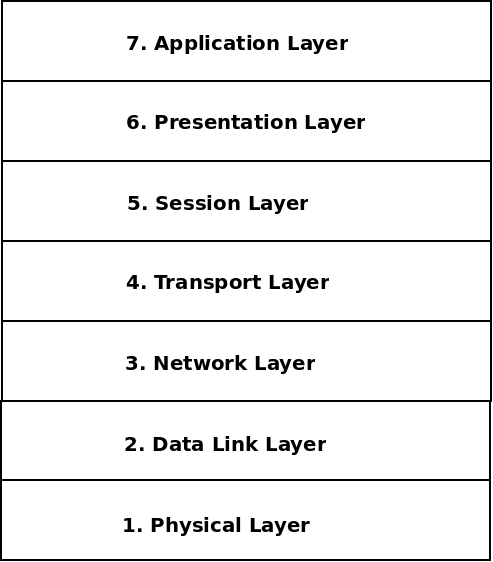
\includegraphics[width=0.8\textwidth]{osi_model}
\end{center}
\caption{OSI model (7-layered)}
\label{fig:osi_model}
\end{figure}

Between each pair of adjacent layers is an interface. The interface defines which 
primitive operations and services the lower layer makes available to the upper one. 
When network designers decide how many layers to include in a network and what 
each one should do, one of the most important considerations is defining clean 
interfaces between the layers. Doing so, in turn, requires that each layer perform 
a specific collection of well-understood functions. In addition to minimizing the 
amount of information that must be passed between layers, clear-cut interfaces 
also make it simpler to replace the implementation of one layer with a completely 
different implementation (eg., all the telephone lines are replaced by satellite 
channels) because all that is required of the new implementation is that it 
offer exactly the same set of services to its upstairs neighbor as the old 
implementation did. In fact, it is common that different hosts use different 
implementations.

While many of the protocols developed within this framework are not greatly used 
today, it remains an interesting academic study for approaches to protocol 
specification. In the original OSI concept in the late 1970s, there would be 
just 6 layers providing (progressively richer) carrier services, with a final 
\emph{application layer} where each specification supported a single end-application, 
with no `holes'.
 
\subsection{Network protocol operations}
Considering the layered model, lower layer network protocol provides services to 
a higher layer protocol. This services are exposed trough protocols interface. 
A protocol then performs certain operations to the point of servicing a higher 
layer protocol which requested a service. For example TCP provides connection-oriented, 
ordered and reliable transfer of data from one TCP endpoint to another, for higher 
level protocol such as \emph{Simple Mail Transfer Protocol} (SMTP) or \emph{File 
Transfer Protocol} (FTP). This is achieved using operations such as \emph{handshaking}, 
\emph{acknowledging} and \emph{signaling}.

A simple protocol operation would be to start the operation and then wait for it 
to complete. But such an approach (called \emph{synchronous} or \emph{blocking} 
operation) would block the progress of a program while the communication is in
progress, leaving system resources idle. The thread of control is blocked within
the function performing the protocol operation, and it can use the result 
immediately after the function returns. This means that the processor can spend 
almost all of its time idle waiting for a certain protocol operation to complete.

Alternatively, it is possible, to start the operation and then perform processing 
that does not require that the operation has completed. This type of operation is 
called \emph{asynchronous} or \emph{non-blocking} operation. Any task that actually 
depends on the operation having completed (this includes both using the return 
values and critical operations that claim to assure that a protocol operation 
at hand has been completed) still needs to wait for the protocol operation to 
complete, and thus is still blocked, but other processing which does not have a 
dependency on the protocol operation can continue. Situations in which a protocol
operation should operate in asynchronous mode are those that can get extremely 
slow, for reasons such as writing or reading from a hard drive (in the context
of network file systems).

Additional issue which needs to be addressed concerning protocol operations is 
the time period in which they must perform. This are called \emph{operation 
timeouts} and they vary a lot and usually depend on the semantics and the 
context of the operation itself.

Further we can separate operations to \emph{passive} and \emph{active}, considering 
if the operation is initiating communication with the other endpoint (eg. active),
or is simply waiting for the communication to be initiated by the other endpoint 
(eg. passive). Also we can utilize terminology such as \emph{server operations} 
and \emph{client operations}, for passive and active operations, respectively.

\subsection{Network protocol data units}
What it boils down to, a protocol operation is actually the exchange of messages.
These messages are transmitted across a virtual communication line between endpoints
or peers that reside on the same layer and thus `speak' the same protocol. 
The abstraction level that the layering approach provides us allows us to think 
of these peers being directly connected. The message that carries the required 
semantics among the protocol peers at hand is called the \emph{protocol data unit}
(PDU).

A PDU in general consists of a header which contains some kind of protocol-control 
information and possibly user data of that layer. The other part is considered 
to be the payload data, formally referred to as \emph{service data unit} (SDU). 
The semantics and syntax of the SDU is known to the higher layer protocol which 
is being serviced by the lower layer protocol. The lower layer protocol has no 
such knowledge and thus SDU is considered as a `hole' to the protocol at hand.

For example in relation to the OSI model layers, the Physical layer PDU is a 
\emph{bit}, the Data Link layer PDU is referred to as a \emph{frame}, while the 
Network layer and the Transport layer use the terms \emph{packet} and 
\emph{segment}, respectively.

PDUs are commonly \emph{binary-based} or \emph{text-based} (also referred to as 
\emph{character-based}). Generally with binary-based PDUs 
protocol gains in speed and bandwidth usage, but in turn has to deal with 
different integer sizes and sign, floating point representations, bit and byte 
ordering. On the other hand text-based PDUs are relatively simple to handle as 
they are most commonly ASCII encoded and thus human-readable and easy debugged.
Of course it's clear that such PDUs are heavy on bandwidth usage. 

\section{Network protocol specification}
Protocols can be (and historically have been) specified in many ways. One 
fundamental distinction is between protocols that utilize character-based PDUs 
versus binary-based PDUs. Such specifications are commonly referred to as 
character-based and binary-based specification, respectively:
\begin{description}
  \item[Character-based specification] The protocol is defined as a series of 
  lines of ASCII encoded text.
  \item[Binary-based specification] The protocol is defined as a string of 
  octets or of bits.
\end{description}

Character-based protocols are often designed as a \emph{command line} or 
\emph{statement-based} protocols. The communication of such protocols consist of 
series of lines of text each of which can be thought of as a command or a 
statement, with textual parameters (frequently comma separated) within each 
command or statement. The examples of such text based protocols are HTTP, FTP, 
POP3, etc. 

The common way of defining a text based protocol is with use of \emph{Backus Naur Form} 
or simply BNF. It is very powerful for defining arbitrary syntactic structures, 
but it does not in itself determine how variable length items are to be delimited 
or iteration counts determined. A part of HTTP specification written in BNF is 
shown in \ref{lst:bnf_http}

\lstset{language=C++}
\lstset{basicstyle=\tiny}
\lstset{caption={BNF specification of HTTP protocol},label=lst:bnf_http}
\lstset{numbers=left, numberstyle=\tiny, stepnumber=1, numbersep=5pt}
\begin{lstlisting}[frame=tb]
SPACE := `` ''
CRLF := ``\r\n''
HTTP-REQUEST := HTTP-REQUEST-LINE HTTP-REQUEST-HEADERS HTTP-MESSAGE-BODY
HTTP-REQUEST-LINE := HTTP-METHOD SPACE HTTP-URI SPACE HTTP-VERSION CRLF
HTTP-METHOD := ``OPTIONS'' | ``GET'' | ``HEAD'' | ``POST'' | ``PUT'' | ``DELETE'' | ``TRACE'' | ``CONNECT''
HTTP-VERSION := ``HTTP/1.0'' | ``HTTP/1.1''
HTTP-REQUEST-HEADERS := HTTP-REQUEST-HEADERS HTTP-REQUEST-HEADER | HTTP-REQUEST-HEADER
HTTP-URI := ...
HTTP-REQUEST-HEADER := ...
HTTP-MESSAGE-BODY := ...
\end{lstlisting}

Binary protocols are more difficult to implement and their wire representation 
is not human-readable, but generally they are more efficient in both bandwidth 
usage and speed. For binary-based specification, approaches vary from various 
\emph{picture-based} methods (\ref{fig:udp_picture_spec}) to use of separately defined notation (syntax) with
associated application-independent encoding rules (serialization protocols).

\begin{figure}[htb]
\begin{center}
\leavevmode
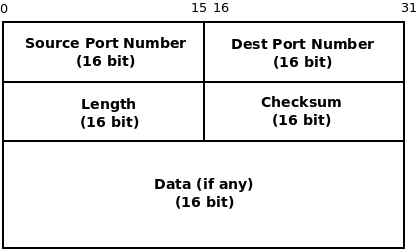
\includegraphics[width=0.8\textwidth]{udp_picture_spec}
\end{center}
\caption{UDP picture-based specification}
\label{fig:udp_picture_spec}
\end{figure}

The later is called the `abstract syntax' approach (\ref{lst:asn_1_foo}). This is the approach taken 
with technologies such as ASN.1, Protocol Buffers, SUN-RPC, ONC-RPC, SOAP etc. 
It has the advantage that it enables designers to produce specifications without 
undue concern with the encoding issues, and also permits application-independent 
tools to be provided to support the easy implementation of protocols specified 
in this way. Moreover, because application-specific implementation code is 
independent of encoding code, it makes it easy to migrate to improved encodings 
as they are developed. 

\lstset{language=Prolog}
\lstset{basicstyle=\tiny}
\lstset{caption={ASN.1 abstract syntax notation example},label=lst:asn_1_foo}
\lstset{numbers=left, numberstyle=\tiny, stepnumber=1, numbersep=5pt}
\begin{lstlisting}[frame=tb]
FooProtocol DEFINITIONS ::= BEGIN
    FooQuestion ::= SEQUENCE {
        trackingNumber INTEGER,
        question       IA5String
    }
    FooAnswer ::= SEQUENCE {
        questionNumber INTEGER,
        answer         BOOLEAN
    }
END
\end{lstlisting}

\subsection{PDU specification}
A PDU is specified using various data types. Let's divide data types into 
\emph{primitive} types or \emph{basic} types and \emph{constructed} types or 
\emph{composite} types. Primitive types include integers, floating point numbers, 
characters, booleans etc. Constructed data types are constructed using primitive 
data types and other constructed types. They provide enclosure for some data type
set. Structures, arrays, strings, unions, enumerators etc., fall into constructed 
data type category.

Different kinds of computers use different conventions for the ordering of bytes 
within data types that are multiple of a byte. Some computers put the most 
significant byte (eg. MSB) within such data type first, this is called 
\emph{`big endian'} order, and others put it last, thus called \emph{`little endian'}
order (eg. LSB). The same goes for bit ordering, all though it's rare to find 
little endian bit ordering into the wild, both on processor architecture and 
network protocol specifications. Integer sizes also differ amongst architectures, 
not to mention floating point representations. Strings have different character 
encodings (ie. character set or simply charset).

So that machines with different conventions and specifications can communicate, 
the network protocol specification must clearly define these attributes to every 
data type transmitted over the network.

Formally we can define integers as a data type which represents some finite 
subset of mathematical integers (integral data type). When specifying an 
integer data type one must consider the following attributes:
\begin{description}
	\item[Size] Most commonly integer sizes are byte multiples, and as such are 
		usually named with the following size specifiers: \emph{char, short, long, long long} or 
		\emph{hyper} respectively pertaining to sizes of 1,2,4,8 bytes. It's not uncommon to 
		define a bit multiple integer size, for instance 13 bits offset field in the 
		IP PDU specification.
	\item[Byte order] Byte order concept is only valid with byte multiple sized 
		data types so only byte sized integers must have byte ordering defined.
		Thus called \emph{byte-sized integers}.
	\item[Bit order] Data types that have size defined as bit multiple are 
		called bit-sized data types, therefor such integers are called 
		\emph{bit-sized integers}. Bit order can be specified for both byte-sized 
		and bit-sized integers. When specified for bit-sized integer the bits are 
		arranged accordingly for the integer as a whole. For byte-sized integers 
		the bit order is considered bytewise and thus is set for each byte.	
	\item[Sign] An integer can be \emph{signed} or \emph{unsigned}. Signed integers
	are stored in a computer using \emph{2's complement}. Distinction must be made 
	as integer operations are different for unsigned versus	signed integers.
\end{description}

In computer science, floating point describes a system for representing real 
numbers which support a wide range of values. The following are the attributes 
applicable to floating point data type:
\begin{description}
	\item[Representation] There are several floating point representations used 
		today in computing. Different processor architectures utilize different 
		representations. These are: \emph{IEEE754, VAX, Cray, IBM}...
	\item[Size] The size of a floating point type is usually determined by it's 
		representation, and most commonly are byte sized.
	\item[Byte order] As a byte-sized data type it must have a defined byte order.
	\item[Bit order] Similar to byte-sized integers bit order is defined bytewise 
		(not as a whole).
\end{description}

One more primitive data type is a character. A character data type is used to 
store symbols such as alphanumeric text, whitespace, punctuation and others. 
These symbols exist at a higher level of abstraction then integers and floating 
point numbers. But similarly to these primitive types, characters also must have 
a mapping from character abstraction to a certain binary representation that can 
be stored in computer memory or transmitted across a network. Essentially a 
character is mapped into an integer data type, so we can use object oriented 
paradigm terminology to describe a character type as being a specialized form of 
an integer type. As such a character inherits all of the mentioned integer data 
type attributes to additionally introducing some of its own:
\begin{description}
	\item[Character set] Also referred to as a \emph{charset, character encoding, 
		character map} or a \emph{code page}. It represents a mapping of symbols 
		into an integer for the purpose of storing these symbols in the computer 
		memory or transmission over the network. These mapping can be either 
		specified using a predefined set of symbol to number conversion (ASCII) 
		or using an encoding algorithm (Unicode).
\end{description}

\section{Abstract and transfer syntax}
The terms \emph{abstract} and \emph{transfer syntax} were primarily developed 
within the OSI work, and are variously used in other related computer disciplines. 
These terms will provide us with the terminology for formally defining Wire 
language and it's purpose.

The following steps are necessary when specifying the messages forming a protocol:
\begin{itemize}
	\item The determination of the information that needs to be transferred in 
		each message. We here refer to this as the semantics associated with the message. 
	\item The design of some form of data-structure (at about the level of generality 
		of a high-level programming language, and using a defined notation) which 
		is capable of carrying the required semantics. The set of values of this 
		data-structure are called the \emph{abstract syntax} of the messages. We call 
		the notation we use to define this data structure or set of values the 
		\emph{abstract syntax notation}.
	\item The crafting of a set of rules for encoding messages such that, given 
		any message defined using the abstract syntax notation, the actual bits 
		on the line to carry the semantics of that message are determined by an 
		algorithm specified once and once only (independent of the application).
		 We call such rules \emph{encoding rules}, and we say that the result of 
		 applying them to the set of messages for a given application defines a 
		 \emph{transfer syntax} for that particular abstract syntax. Therefor, 
		 a transfer syntax is the set of bit-patterns to be used to represent 
		 the abstract values in the abstract syntax, with each bit-pattern 
		 representing just one \emph{abstract value}.
\end{itemize}

So to simplify a little bit, let's say, for example, that we wish to make a 
notation to declare an integer type and assign it a value. To that point let us 
borrow the notation that C language uses or simply:
\lstset{language=C}
\lstset{basicstyle=\tiny}
\lstset{caption={C abstract syntax notation},label=lst:c_int}
\lstset{numbers=left, numberstyle=\tiny, stepnumber=1, numbersep=5pt}
\begin{lstlisting}[frame=tb]
int a = 1;
\end{lstlisting}

We can now say that the value `1' is an abstract value that represents an integer 
value. The set of these abstract values (ie. {...-1, 0, 1, 2, 3, 4, 5, 6, 7...}) 
is called the abstract syntax. The notation used to declare and define an instance 
of an abstract syntax is called an abstract syntax notation.

The usage of term `abstract' is totally justified, considering we are dealing 
with the abstraction of integers, floating point numbers, characters etc.
The representation used to store an abstract syntax in computer memory is called
the \emph{concrete syntax}. For example IEEE754 floating point representation is
one of the concrete syntaxes for storing floating point numbers. 

Abstract syntaxes should be independent of the concrete syntaxes which can and 
usually do differ amongst different machines.

The transfer syntax is the representation used to transfer the abstract syntax 
over the communication line. A certain instance of the abstract syntax or the 
abstract value must have a unique transfer value so it can be restored on the 
other endpoint. The transfer syntax must take in order the differences in concrete
syntaxes between communicating peers, therefore the transfer syntax must correspond
to some sort of protocol. The protocol or algorithm or encoder or whatever you 
might call it, which maps the abstract syntax to a corresponding transfer syntax 
or even a concrete syntax, which carries its semantics, is called 
\emph{serialization}.

\begin{figure}[htb]
\begin{center}
\leavevmode
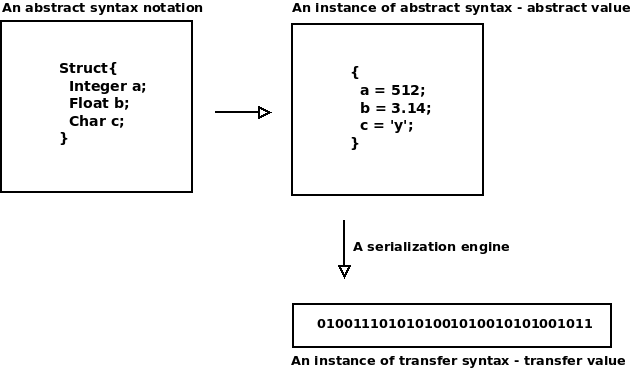
\includegraphics[width=0.8\textwidth]{syntax_relations}
\end{center}
\caption{Syntax relations}
\label{fig:syntax_relations}
\end{figure}

The figure \ref{fig:syntax_relations} illustrates the mentioned concepts and 
their relations. 

What's left is to list some technologies and formally describe them using these 
newly learned terminology.
First lets mention the \emph{Abstract Syntax Notation One} technology (ASN.1), 
which is, as you may noticed, named quite literal. Some of the abstract data 
types that the ASN.1 provides are:
\begin{enumerate}
	\item Basic (primitive) types \emph{boolean, integer, real, enumerated, bit string, 
	octet string, null} \ldots
	\item Constructed types include \emph{sequence, set, choice}...
\end{enumerate}

The ASN.1 is an abstract syntax notation which uses several different serialization 
protocols to produce the transfer syntax:
\begin{enumerate}
	\item Basic Encoding Rules (BER)
	\item Canonical Encoding Rules (CER)
	\item Distinguished Encoding Rules (DER)
	\item XML Encoding Rules (XER)
	\item Packed Encoding Rules (PER)
	\item Generic String Encoding Rules (GSER)
\end{enumerate}

Other popular technology that is utilized by the SUN-RPC remote procedure call
protocol is the \emph{External Data Representation} (XDR). XDR also includes 
an abstract syntax notation that defines basic data types such as \emph{integer 
and hyper, float and double, quadruple, bool} and constructed data types such 
as \emph{structures, enumerations and unions}. The serialization for each data 
type is specified in RFC4506.

\emph{JavaScript Object Notation} or simply JSON is widely known and popular 
data interchange technology used in Web today. It consists of an abstract syntax 
notation that is a subset of JavaScript scripting language. All though its main 
purpose is the serialization and transmission of JavaScript objects between a 
server and a web application (client), JSON is language independent. 
The serialized objects,aka the transfer syntax, is in human-readable text form.

\section{Wire formal definition}
By using the terminology and concepts elaborated in the previous sections, we will 
formally define the Wire project. First of all Wire is a computer language, more 
precisely a subset which is called a \emph{definition language}. It's a 
\emph{domain-specific} or a \emph{special-purpose} language (we'll get to that 
later on), oppose to general-purpose languages such as C or Java. Also, to specify 
a bit deeper, Wire provides an abstract syntax notation.

The idea behind Wire is to provide a language which is used to describe/define 
(ie. definition language) the \emph{on the wire representation} of an 
arbitrary network protocol. One could say that Wire is used to define the transfer 
syntax for some protocol. So an abstract syntax notation for describing a transfer syntax.

Wire language compiler takes a specification of a certain protocol written in 
Wire and produces code that handles the defined protocol. By that I mean generates 
code to easily build and dissect protocol data units as well as handle all of the 
defined protocol operations.

\section{Wire overview}
For the sake of demonstrating Wire, we will develop a custom network protocol. 
The development process and the making of the final specification will help us 
explain the purpose and the inner workings of Wire. Also it will show us some 
general guidelines and steps needed when designing a protocol.

So let's call this new network protocol \emph{`Math'}, it will resemble a remote 
procedure call protocol which will offer a mathematical service. 
So we've already defined:
\begin{enumerate}
	\item Name - `Math'
	\item Service - Mathematical operations.
\end{enumerate}

So let's start writing a Wire definition of our `Math' protocol. 
This is the simplest protocol definition in Wire:
\lstset{language=IDL}
\lstset{basicstyle=\tiny}
\lstset{caption={Wire example - Designing `Math' (step 1)},label=lst:mat_step_1}
\lstset{numbers=left, numberstyle=\tiny, stepnumber=1, numbersep=5pt}
\begin{lstlisting}[frame=tb]
[
  //protocol attributes
] protocol Math{
  //data type definitions
  //operation declarations
}
\end{lstlisting}

This represents nothing yet, but be patient...we'll get there. First we can notice 
line comments similar to those found in C syntax. Second thing to notice is the 
\emph{`protocol'} keyword which is used to define a new protocol named `Math'. 
What precedes this keyword is a pair of square brackets. These will hold a list 
of attributes that are applicable to a protocol definition. Actually every Wire 
component can have attributes applied to it, which attributes are applicable 
where we'll learn gradually.

Let's define our service a bit more. So we wish to provide basic mathematical 
operations such as addition, subtraction, multiplication, division and power:

\lstset{language=IDL}
\lstset{basicstyle=\tiny}
\lstset{caption={Wire example - Designing `Math' (step 2)},label=lst:mat_step_2}
\lstset{numbers=left, numberstyle=\tiny, stepnumber=1, numbersep=5pt}
\begin{lstlisting}[frame=tb]
[
  //protocol attributes
] protocol Math{
  //data type definitions
  //operation declarations
  operation Add();
  operation Sub();
  operation Mul();
  operation Div();
  operation Pow();
}
\end{lstlisting}

The \emph{`operation'} keyword is assigned the honor of declaring our protocol 
operations. Currently these operations are dumb as they have an empty arguments 
list. The operation declaration can only have arguments of \emph{`pdu'} data type.
This is reasonable as an operation is the exchange of messages between peers, 
these messages are called protocol data units and the `pdu' data type embodies 
this concept in Wire.

So a pdu definition is defined using the \emph{`pdu'} keyword. I decided to 
define one general PDU that can capture all of the required semantics. I called 
it `Math' protocol data unit. One could decide to go with, for example, two PDUs, 
one which will carry the request information and the other that will hold the 
response information. Notice that this is a design issue and as such falls under 
personal preference.

\lstset{language=IDL}
\lstset{basicstyle=\tiny}
\lstset{caption={Wire example - Designing `Math' (step 3)},label=lst:mat_step_3}
\lstset{numbers=left, numberstyle=\tiny, stepnumber=1, numbersep=5pt}
\begin{lstlisting}[frame=tb]
[
  //protocol attributes
] protocol Math{
  //data type definitions
  pdu Math{};
  //operation declarations
  operation Add([push] pdu Math math_req, [pull] pdu Math math_rep);
  operation Sub([push] pdu Math math_req, [pull] pdu Math math_rep);
  operation Mul([push] pdu Math math_req, [pull] pdu Math math_rep);
  operation Div([push] pdu Math math_req, [pull] pdu Math math_rep);
  operation Pow([push] pdu Math math_req, [pull] pdu Math math_rep);
}
\end{lstlisting}

Now our operations have a valid argument list. Each pdu local declaration in the 
argument list has been applied an attribute. These \emph{`push'} and \emph{`pull}
attributes are only applicable to pdu declarations that are placed in the argument 
list of an operation declaration:
\begin{description}
	\item[push] It's a notion used to define that a pdu is being sent to the 
		carrier service which conveys it to the other endpoint. The carrier 
		service is situated at a lower layer, so the PDU is virtually being 
		\emph{`pushed'} down.
	\item[pull] Similar to `push', with the exception that the pdu is being 
		received from the other endpoint, or \emph{`pulled'} up from the lower 
		layer protocol.
\end{description}

Each operation pushes one pdu, similar to function arguments, and pulls one, ie. 
function return value. Obviously these pdus must be designed so that are able to 
carry all the required information such as integer number and/or real number 
arguments, result of the mathematical operation and quite possibly some sort of 
error messages that indicate an exception (for example division by zero).

\lstset{language=IDL}
\lstset{basicstyle=\tiny}
\lstset{caption={Wire example - Designing `Math' (step 4)},label=lst:mat_step_4}
\lstset{numbers=left, numberstyle=\tiny, stepnumber=1, numbersep=5pt}
\begin{lstlisting}[frame=tb]
[
  //protocol attributes
] protocol Math{

  //data type definitions
  enum PDUType{ 
    REQUEST = 0, 
    REPLY = 1 
  }; 

  struct MathReq {};

  struct MathRep{};

  pdu Math{
    enum PDUType epdu_type; 
    union <epdu_type> { 
      case REQUEST: 
        struct MathReq smathreq; 
      case REPLY: 
        struct MathRep smathrep; 
      default: 
        exception("epdu_type: value not used"); 
    }; 
  };

  //operation declarations
  operation Add([push] pdu Math math_req, [pull] pdu Math math_rep);
  operation Sub([push] pdu Math math_req, [pull] pdu Math math_rep);
  operation Mul([push] pdu Math math_req, [pull] pdu Math math_rep);
  operation Div([push] pdu Math math_req, [pull] pdu Math math_rep);
  operation Pow([push] pdu Math math_req, [pull] pdu Math math_rep);
};
\end{lstlisting}

We extended our \emph{`Math'} pdu with the \emph{union} construct which allows us 
to define conditional structuring. A union declaration has a \emph{switch} which 
determines the proper structure at runtime. The switch value is used to check 
the equality of \emph{case}s so the code can unambiguously process the structure.
This particular union declaration instance is an example of the, so called, 
\emph{anonymous} union declaration, oppose to a \emph{named} union declaration. 

Another handy data type we introduced with this progress is the enumeration data 
type. It's no novelty, but it's usage results in more elegant definitions. 
The enum definition takes a list of names (ie. identifiers) for integer constants 
who will later on be referenced by that name.

Our \emph{`Math'} pdu definition is now equipped with sufficient information to 
carry both the request and response information. We've reached the second checkpoint 
in designing a network protocol:
\begin{enumerate}
	\item Interface – We've designed the exact interface to our mathematical 
		service. It consists of operations: \emph{Add, Sub, Mul, Div, Pow}.
	\item PDU – Decided on the structure of the protocol data units. Preferred 
		on a single PDU definition that can carry a more general information.
\end{enumerate}

What's next is to exactly define the information that will be carried within 
request and reply structures. So we introduce the structure definition notation 
with the \emph{`struct'} keyword. Syntactically it's no different from the pdu definition.
Another primitive type used is the string defined using the \emph{`string'} 
keyword. We used it to carry the error message.
\lstset{language=IDL}
\lstset{basicstyle=\tiny}
\lstset{caption={Wire example - Designing `Math' (step 5)},label=lst:mat_step_5}
\lstset{numbers=left, numberstyle=\tiny, stepnumber=1, numbersep=5pt}
\begin{lstlisting}[frame=tb]
[
  //protocol attributes
] protocol Math{

  //data type definitions
  enum PDUType{ 
    REQUEST = 0, 
    REPLY = 1 
  }; 
  
  enum ReplyType{ 
    FAILURE, 
    SUCCESS
  }; 

  enum NumberType{ 
    INTEGER, 
    REAL 
  }; 

  struct MathReq {
    enum NumberType enumber_type; 
    unsigned int narguments; 
    union <enumber_type> { 
      case INTEGER: 
        unsigned int size_arg; 
        signed int sint_args[narguments]; 
      case FLOAT: 
        unsigned int size_arg; 
        float fp_args[narguments] ;
      default: 
        exception("enumber_type: value not used"); 
    };
  };

  struct MathRep{
    enum ReplyType ereply_type; 
    union <ereply_type>{ 
      case FAILURE: 
        string   strerror; 
      case SUCCESS: 
        enum NumberType enumber_type; 
        union <enumber_type> { 
          case INTEGER: 
            unsigned int size_res; 
            signed int sint_res;   
          case REAL: 
            unsigned int size_res; 
            float fp_args
          default: 
            exception("enumber_type: value not used"); 
      };
    default: 
      exception("enumber_type: value not used"); 
    };
  };

  pdu Math{
    enum PDUType epdu_type; 
    union <epdu_type> { 
      case REQUEST: 
        struct MathReq smathreq; 
      case REPLY: 
        struct MathRep smathrep; 
      default: 
        exception("epdu_type: value not used"); 
    }; 
  };

  //operation declarations
  operation Add([push] pdu Math math_req, [pull] pdu Math math_rep);
  operation Sub([push] pdu Math math_req, [pull] pdu Math math_rep);
  operation Mul([push] pdu Math math_req, [pull] pdu Math math_rep);
  operation Div([push] pdu Math math_req, [pull] pdu Math math_rep);
  operation Pow([push] pdu Math math_req, [pull] pdu Math math_rep);
};
\end{lstlisting}

Notice the \emph{exception} statement. It's a Wire construct used to designate 
an exception state of some kind. This \emph{function call} like statement takes 
variable length list of arguments that are passed to the runtime that will 
eventually handle the exception at hand. What's considered an exception is decided 
by the protocol designer. I used it to designate the occurrence of invalid value.

At this point we've, semantically, fully defined the protocol from an abstraction 
level that only deals with information and its exchange trough operations. 
Needless to say we've defined the abstract syntax of the Math protocol. 
In the process we've encountered every Wire component: \emph{protocol definition, 
operation declarations and data type definitions}. 
Primitive data types: \emph{integers, floats and strings} and constructed data 
types: \emph{protocol data units, structures, unions, arrays and enumerations}.

Now it's time to define and utilize the Wire attribute concept to exactly define 
the on the wire representation of the protocol at hand. Attributes can be applied 
to every Wire component. They are used to semantically link scope related objects,
define sanity checks and to give instructions to both the Wire serialization engine 
and the communication engine. One could say that by using attributes you can 
exactly define the transfer syntax of a protocol.

First let's talk to the communication engine. What we need to define for Math 
protocol is the carrier service. The carrier service is a lower layer protocol 
which is assigned the job of carrying the Math PDUs to the other Math endpoint.
To decide on the carrier service for Math, I took into consideration the following:
\begin{enumerate}
	\item Math endpoints must be able to communicate over the IP networks.
	\item The information exchanged over the wire is sensitive in a way that it 
		must be correctly transported to the other side, thus we want reliable 
		and ordered transport service.
\end{enumerate}

So a common practice when met with such requirements is to choose the 
\emph{Transmission Control Protocol}. TCP resides on top of the IP protocol and 
uses the \emph{port} addressing concept to deliver data from one process to another. 
So let's choose our port number to be 31337 (elitenzi).

Wire uses the \emph{endpoint} attribute for defining protocol endpoint information. 
Generally endpoint attribute takes a name and the addressing information of the 
carrier protocol. Note that a protocol can specify any number of carrier services, 
but practically it depends on the communication engine and what services it supports.

\lstset{language=IDL}
\lstset{basicstyle=\tiny}
\lstset{caption={Wire example - Designing `Math' (step 6)},label=lst:mat_step_6}
\lstset{numbers=left, numberstyle=\tiny, stepnumber=1, numbersep=5pt}
\begin{lstlisting}[frame=tb]
[
  //protocol attributes
  endpoint(``tcp:31337''),
  size(4),
  byte_order(``MSB''),
  bit_order(``MSB'')
] protocol Math{

  //data type definitions
  [size(1)] enum PDUType{ 
    REQUEST = 0, 
    REPLY = 1 
  }; 
  
  enum ReplyType{ 
    FAILURE, 
    SUCCESS
  }; 

 enum NumberType{ 
    INTEGER, 
    REAL 
  }; 

  struct MathReq {
    enum NumberType enumber_type; 
    [size(2), byte_order(``LSB'')] unsigned int narguments; 
    union <enumber_type> { 
      case INTEGER: 
        [range(1,32)] unsigned int size_arg; 
        [size_bits(size_arg)] signed int sint_args[narguments]; 
      case FLOAT: 
        [list(32,64)] unsigned int size_arg; 
        [size_bits(size_arg), fp_rep(``IEEE754'')] float fp_args[narguments] ;
      default: 
        exception("enumber_type: value not used"); 
    };
  };

  struct MathRep{
    enum ReplyType ereply_type; 
    union <ereply_type>{ 
      case FAILURE: 
        [charset(``ASCII''), delimiter(``\0'')] string   strerror; 
      case SUCCESS: 
        enum NumberType enumber_type; 
        union <enumber_type> { 
          case INTEGER: 
            [range(1,32)] unsigned int size_res; 
            [size_bits(size_res)] signed int sint_res;   
          case REAL: 
            [list(32,64)] unsigned int size_res; 
            [size_bits(size_res), fp_rep(``IEEE754'')] float fp_args 
          default: 
            exception("enumber_type: value not used"); 
      };
    default: 
      exception("enumber_type: value not used"); 
    };
  };

  pdu Math{
    enum PDUType epdu_type; 
    union <epdu_type> { 
      case REQUEST: 
        struct MathReq smathreq; 
      case REPLY: 
        struct MathRep smathrep; 
      default: 
        exception("epdu_type: value not used"); 
    }; 
  };

  //operation declarations
  [timeout(5)] operation Add([push] pdu Math math_req, [pull] pdu Math math_rep);
  [timeout(5)] operation Sub([push] pdu Math math_req, [pull] pdu Math math_rep);
  [timeout(5)] operation Mul([push] pdu Math math_req, [pull] pdu Math math_rep);
  [timeout(5)] operation Div([push] pdu Math math_req, [pull] pdu Math math_rep);
  [timeout(5)] operation Pow([push] pdu Math math_req, [pull] pdu Math math_rep);
};
\end{lstlisting}

The timeout attribute takes the number of seconds as the sole argument, and is 
applicable to operation objects. This states the maximum amount of time that the 
operation has to finish, timing from the invocation moment. If the operations has 
failed to do so for whatever reason the timeout exception is raised and handled 
by the application logic.

The \emph{attributes applicability} is defined as the context in which the attribute 
is valid, or equally as the list of objects that are directly influenced by the 
attribute. For example the floating point representation attribute (\emph{`fp\textunderscore{}rep'})
 is applicable only to float local declarations, oppose to integer local declarations. 
An attribute can be defined as a \emph{general attribute}, which is useful for 
general application. So for example if we define byte order attribute 
(\emph{`byte\textunderscore{}order'}) in the protocol definition attribute list it means that 
every enclosed object receives this attribute (except when overriden by a more 
specific attribute statement).

We've defined a few general attributes for the Math protocol. We've set the 
general byte order and bit order to big endian, while defining the default 
primitive size to 4 bytes.

We've listed a few of the command attributes that are used to define the transfer 
syntax of our protocol, by commanding the serialization and the communication engine. 
There are also attributes that define certain semantic checks that must be performed 
for a given object at runtime. Range and list check for integer and float 
declarations are example of such attributes. 

\section{Wire lexical conventions}
Lexical analysis is the process of converting a sequence of characters into a 
sequence of lexical units called \emph{tokens}. Wire uses \emph{GNU Flex} tool 
to generate the Wire tokenizer. Flex is really convenient for processing textual 
files as it allows users to simply describe tokens using regular expressions. 
Appendix \ref{lst:wire_l} holds the flex source file which lists all of the defined 
Wire tokens and their corresponding regular expressions.

Let's introduce some, more relevant, lexical conventions for Wire users. The 
following lists the reserved words:
\lstset{language=IDL}
\lstset{basicstyle=\footnotesize}
\lstset{caption={Wire keywords},label=lst:wire_keywords}
\lstset{numbers=left, numberstyle=\tiny, stepnumber=1, numbersep=5pt}
\begin{lstlisting}[frame=tb]
byte	enum	operation
uint	struct	import
sint	union	typedef
float	pdu	default
string	protocol
\end{lstlisting}

A Wire identifier follows C syntax rules, so the following are valid examples of 
Wire identifiers:
\lstset{language=IDL}
\lstset{basicstyle=\footnotesize}
\lstset{caption={Wire identifier},label=lst:wire_identifier}
\lstset{numbers=left, numberstyle=\tiny, stepnumber=1, numbersep=5pt}
\begin{lstlisting}[frame=tb]
ident1234
ident_1234
ident1234_
_ident1234
\end{lstlisting}

A valid character set for a Wire identifier consists of alphanumeric Al characters
and the underscore. Note that the first character must be a letter or an 
underscore sign.

The last thing that's left are the numeric constants and the string constants. 
Integer constants can be stated in decimal, hexadecimal, binary and octal form:
\lstset{language=IDL}
\lstset{basicstyle=\footnotesize}
\lstset{caption={Wire integer constants},label=lst:wire_int_const}
\lstset{numbers=left, numberstyle=\tiny, stepnumber=1, numbersep=5pt}
\begin{lstlisting}[frame=tb]
255
0xFF or 0xff
0377
0b11111111
\end{lstlisting}

Floating point number constants look like:
\lstset{language=IDL}
\lstset{basicstyle=\footnotesize}
\lstset{caption={Wire floating point constants},label=lst:wire_fp_const}
\lstset{numbers=left, numberstyle=\tiny, stepnumber=1, numbersep=5pt}
\begin{lstlisting}[frame=tb]
3.14
3.14e10
3.14E10
3.14e-10
\end{lstlisting}

The `e' or `E' notation is used for defining an exponent.
A string constant is enclosed between the two double apostrophe signs:
\lstset{language=IDL}
\lstset{basicstyle=\footnotesize}
\lstset{caption={Wire string constants},label=lst:wire_str_const}
\lstset{numbers=left, numberstyle=\tiny, stepnumber=1, numbersep=5pt}
\begin{lstlisting}[frame=tb]
``This is a string constant''
``Wire uses the \\ as the escape symbol''
\end{lstlisting}
Wire string constants follow the same rules of C strings.

\begin{figure}[htb]
\begin{center}
\leavevmode
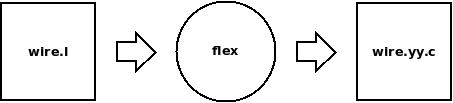
\includegraphics[width=0.8\textwidth]{flex}
\end{center}
\caption{Wire tokenizer compilation process}
\label{fig:wire_tknzr_flex}
\end{figure}

\ref{fig:wire_tknzr_flex} shows the compilation process which generates the Wire 
tokenizer code. The Flex tool takes a \emph{`wire.l'} file as the input. 
This file holds token descriptions written in Flex syntax. Flex processes this 
file and produces the actual C code that does the lexical analysis, \emph{`wire.yy.c'}.
The output file contains \emph{`yylex()'} function which upon invocation returns 
the next token in the assigned stream.

\section{Wire syntax}
Parsing or formally syntax analysis is  the process of analyzing a text, made of 
a sequence of tokens (for example, words), to determine its grammatical structure 
with respect to a given (more or less) formal grammar. Wire utilizes the 
\emph{GNU Bison} tool which reads a specification of a context-free language, 
warns about any parsing ambiguities, and generates a parser in C which reads 
sequences of tokens and decides whether the sequence conforms to the syntax 
specified by the grammar. Bison generates LALR parsers.

\begin{figure}[htb]
\begin{center}
\leavevmode
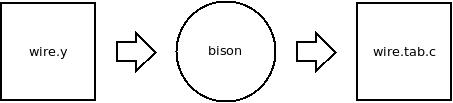
\includegraphics[width=0.8\textwidth]{bison}
\end{center}
\caption{Wire parser compilation process}
\label{fig:wire_prsr_bison}
\end{figure}

Figure \ref{fig:wire_prsr_bison} demonstrates the translation process which 
generates the Wire parser code. Bison input is a \emph{`wire.y'} file which 
contains the syntax definition written in Bison variance of BNF syntax definition 
notation. File \emph{`wire.tab.c'} contains the C code that implements the parsing 
logic for our language.

My intention was to make Wire syntax simple and intuitive, clean and easy memorable. 
Appendix \ref{lst:wire_syn_bnf} contains a numbered list of all Wire grammar rules. 

This chapter holds a brief explanation for every syntactical grouping found in Wire syntax.

The top level grouping is a protocol grouping, and is defined as follows:
\lstset{language=IDL}
\lstset{basicstyle=\tiny}
\lstset{caption={Wire protocol definition},label=lst:wire_proto_def}
\begin{lstlisting}[frame=tb]
    3 protocol: attribute_list_opt tPROTOCOL tIDENTIFIER '{' protocol_body_opt '}'
    4 protocol_body_opt: protocol_body
    5                  | /* empty */
    6 protocol_body: protocol_body_component ';'
    7              | protocol_body protocol_body_component
    8 protocol_body_component: type_definition
    9                        | operation_declarator
\end{lstlisting}

The \emph{`tPROTOCOL'} token represents the \emph{`protocol'} keyword and 
\emph{`tIDENTIFIER'} token the identifier lexical unit. The protocol body is 
constructed of components that are separated by a semicolon (`;'). These components 
can be a type definition or a operation declaration. Notice that the protocol 
definition is prepended an optional attribute syntactical grouping:
\lstset{language=IDL}
\lstset{basicstyle=\tiny}
\lstset{caption={Wire attribute list},label=lst:wire_attr_lst}
\begin{lstlisting}[frame=tb]
   10 attribute_list_opt: '[' attribute_list ']'
   11                   | /* empty */
   12 attribute_list: attribute
   13               | attribute_list ',' attribute
   14 attribute: tIDENTIFIER
   15          | tIDENTIFIER '(' attribute_argument_list ')'
   16 attribute_argument_list: attribute_argument
   17                        | attribute_argument_list ',' attribute_argument
   18 attribute_argument: const_exp
\end{lstlisting}

The attribute list construct is surrounded by the square brackets. An attribute 
can be specified in one of two forms: with arguments or without arguments. 
When specified with arguments, these arguments are comma separated and must 
resolve to syntactical grouping that represents the constant expression.
\lstset{language=IDL}
\lstset{basicstyle=\tiny}
\lstset{caption={Wire type definition},label=lst:wire_type_def}
\begin{lstlisting}[frame=tb]
   19 type_definition: enum_definition
   20                | union_definition
   21                | struct_definition
   22                | pdu_definition   
\end{lstlisting}

The type definition groups rules for definitions of enumerator, union, structure 
and protocol data unit constructs. The enumerator definition looks like:
\lstset{language=IDL}
\lstset{basicstyle=\tiny}
\lstset{caption={Wire enumerator definition},label=lst:wire_enum_def}
\begin{lstlisting}[frame=tb]
   23 enum_definition: attribute_list_opt tENUM tIDENTIFIER '{' enum_body '}'
   24 enum_body: enum_body_component
   25          | enum_body ',' enum_body_component
   26 enum_body_component: tIDENTIFIER '=' const_exp
   27                    | tIDENTIFIER
\end{lstlisting}

As expected the optional attribute list precedes the enumerator definition. The 
\emph{`tENUM'} token represents the \emph{`enum'} keyword. Enumerator body 
components are comma separated and can be specified in one of two forms: 
with or without explicit value assignment. If no explicit assignment  is specified, 
for a component, the numbering or indexing is calculated considering the offset 
from last of such assignment (or from zero if no assignment is specified).
\lstset{language=IDL}
\lstset{basicstyle=\tiny}
\lstset{caption={Wire union definition},label=lst:wire_union_def}
\begin{lstlisting}[frame=tb]
   28 union_definition: attribute_list_opt tUNION tIDENTIFIER '{' union_body '}'
   29 union_body: union_body_component
   30           | union_body union_body_component
   31 union_body_component: const_exp ':' local_declarator_list
   32                     | tDEFAULT ':' local_declarator_list 
\end{lstlisting}

The union component is a defined as a case component. The case is a constant 
expression which is followed by a group of local declarations. The union switch 
is defined on union declaration. Its purpose is to provide a notation for 
conditional processing in Wire by checking the equivalence with the listed case 
constant expressions.

A structure body consists of local declarations separated by a semicolon:
\lstset{language=IDL}
\lstset{basicstyle=\tiny}
\lstset{caption={Wire structure definition},label=lst:wire_struct_def}
\begin{lstlisting}[frame=tb]
   33 struct_definition: attribute_list_opt tSTRUCT tIDENTIFIER '{' struct_body '}'
   34 struct_body: struct_body_component
   35            | struct_body struct_body_component
   36 struct_body_component: local_declarator ';'
\end{lstlisting}

Syntactically there is no difference between a structure definition and a protocol 
data unit definition:
\lstset{language=IDL}
\lstset{basicstyle=\tiny}
\lstset{caption={Wire pdu definition},label=lst:wire_pdu_def}
\begin{lstlisting}[frame=tb]
   37 pdu_definition: attribute_list_opt tPDU tIDENTIFIER '{' pdu_body '}'
   38 pdu_body: pdu_body_component
   39         | pdu_body pdu_body_component
   40 pdu_body_component: local_declarator ';'
\end{lstlisting}

Next lets look at the local declarator construct:
\lstset{language=IDL}
\lstset{basicstyle=\tiny}
\lstset{caption={Wire local declarators},label=lst:wire_local_decl}
\begin{lstlisting}[frame=tb]
   41 local_declarator: primitive_local_declarator
   42                 | constructed_local_declarator
   43                 | anon_local_declarator
   44 local_declarator_list: local_declarator ';'
   45                      | local_declarator_list local_declarator ';'
   46 primitive_local_declarator: attribute_list_opt tBYTE tIDENTIFIER array_declarator_opt
   47                           | attribute_list_opt tFLOAT tIDENTIFIER array_declarator_opt
   48                           | attribute_list_opt tSTRING tIDENTIFIER array_declarator_opt
   49                           | attribute_list_opt tUINT tIDENTIFIER array_declarator_opt  
   50                           | attribute_list_opt tSINT tIDENTIFIER array_declarator_opt  
   51 constructed_local_declarator: attribute_list_opt tENUM tIDENTIFIER tIDENTIFIER array_declarator_opt
   52                             | attribute_list_opt tSTRUCT tIDENTIFIER tIDENTIFIER array_declarator_opt
   53                             | attribute_list_opt tUNION tIDENTIFIER tIDENTIFIER array_declarator_opt 
   54                             | attribute_list_opt tPDU tIDENTIFIER tIDENTIFIER array_declarator_opt   
   55 anon_local_declarator: attribute_list_opt tUNION '<' const_exp '>' '{' union_body '}'
   56 array_declarator_opt: '[' const_exp ']'
   57                     | /* empty */
\end{lstlisting}

A local declaration includes a primitive, constructed and anonymous local declarator.
The term \emph{`local'} is used to denote the scope of declared objects. 
A primitive local declaration is simply a declaration of object that is of 
primitive type (such as string or integer). Similarly the constructed declaration 
is a declaration of an object that is of some constructed data type (for example structure). 
The anonymous local declaration, oppose to a named declaration, is a handy 
syntactical construct used to declare an union local declaration without a 
\emph{`name'}.

All of the declarations can be appended an array declarator which takes a constant 
expression to denote the size of the array.
Finally, what does the constant expression look like:
\lstset{language=IDL}
\lstset{basicstyle=\tiny}
\lstset{caption={Wire local declarators},label=lst:wire_const_exp}
\begin{lstlisting}[frame=tb]
   62 const_exp: integer_const_exp
   63          | float_const_exp 
   64          | string_const_exp
   65          | identifier
   66          | arithmetic_exp
   67          | relational_exp
   68          | logical_exp
   69          | bitwise_exp
   70 float_const_exp: tFLOATCONST
   71 string_const_exp: tSTRINGCONST
   72 integer_const_exp: tINTCONST
   73 arithmetic_exp: const_exp '+' const_exp
   74               | const_exp '-' const_exp
   75               | const_exp '*' const_exp
   76               | const_exp '/' const_exp
   77               | const_exp '%' const_exp
   78 relational_exp: const_exp '>' const_exp
   79               | const_exp '<' const_exp
   80               | const_exp tRELEQU const_exp 
   81               | const_exp tRELNEQU const_exp
   82               | const_exp tRELGE const_exp
   83               | const_exp tRELLE const_exp
   84 logical_exp: '!' const_exp
   85            | const_exp tLOGAND const_exp
   86            | const_exp tLOGOR const_exp
   87 bitwise_exp: '~' const_exp
   88            | const_exp '&' const_exp   
   89            | const_exp '|' const_exp   
   90            | const_exp '^' const_exp   
   91            | const_exp tBITSR const_exp
   92            | const_exp tBITSL const_exp
   93 identifier: tIDENTIFIER
   94           | identifier '.' tIDENTIFIER
\end{lstlisting}

As we can see a constant expression expands to several expressions. So we have 
constant expression for primitive types, such as integers, floating point numbers 
and strings. There is an identifier expression which must resolve to certain object 
declared in a related scope. Furthermore Wire provides arithmetic, relational, 
logical and bitwise expressions.
\lstset{language=IDL}
\lstset{basicstyle=\tiny}
\lstset{caption={Wire operation declarator},label=lst:wire_op_decl}
\begin{lstlisting}[frame=tb]
   58 operation_declarator: attribute_list_opt tOPERATION tIDENTIFIER '(' operation_arg_list ')'
   59 operation_arg_list: operation_arg ','
   60                   | operation_arg_list operation_arg
   61 operation_arg: attribute_list tPDU tIDENTIFIER tIDENTIFIER
\end{lstlisting}
The operation declaration construct, similar to function declaration construct
found in other languages, receives an comma separated argument list. Syntax enforces
that argument list of an operation contains only pdu object local declarations.

After a successful reduction of our input Wire definition to the starting parsing 
symbol an abstract syntax tree is created for that particular Wire definition 
instance. This abstract syntax tree is passed over to the next step of the 
language analysis, the semantic check.

\section{Wire semantics}
The semantic check stage of Wire language analysis consists of several logically divided phases:
\begin{itemize}
	\item Attribute check – involves attribute arguments check and attribute applicability check.
	\item Local declaration scope check.
	\item Data type definition and operation declaration name check.
	\item Constant expression check.
\end{itemize}

Of course before any of that is possible, we must first formally define the Wire 
attribute concept and the related terminology:
\begin{wiredef}
Attribute is a Wire construct or a notation used to provide semantic extensions 
the language components and to specify instructions to both the Wire serialization 
engine and communication engine.
\end{wiredef}

Attribute is said to be applied to a certain Wire component:
\begin{wiredef}
Attribute applicability is defined as the context in which the attribute is valid, 
or equally as the list of Wire components that are directly influenced by the attribute.
\end{wiredef}

For example the floating point representation attribute is applicable only to 
floating point number declarations, oppose to, for example, integer declarations.

I decided to introduce yet another attribute concept, which comes in quite handy:
\begin{wiredef}
A general attribute is an attribute that can be placed in the attribute list of 
a Wire component that has no applicability relation to that attribute.
\end{wiredef}

This allows us to define such attribute in a more general context. So for example 
if we define byte order attribute in the protocol definition attribute list it 
means that every enclosed component, implicitly, receives this attribute (except 
when overriden by a more specific attribute definition).

\begin{description}
	\item[byte\textunderscore{}order(string)] General serialization attribute applicable to uint,sint,float,string local declarations.
	\item[bit\textunderscore{}order(string)] General serialization attribute applicable to uint,sint,float,string local declarations.
	\item[fp\textunderscore{}rep(string)] General serialization attribute applicable to float local declarations.
	\item[char\textunderscore{}enc(string)] General serialization attribute applicable to string local declarations.
	\item[size(uint)] General serialization attribute applicable to uint,sint,float,string local declarations.
	\item[size\textunderscore{}bits(uint)] General serialization attribute applicable to uint,sint,float,string local declarations.
	\item[align(uint)] Non-general serialization attribute applicable to any local declaration and any type definition.
	\item[delimiter(any)] Non-general serialization attribute applicable to array and string declarations.
	\item[endpoint(string)] Non-general communication attribute applicable to protocol definition.
	\item[timeout(uint)] General communication attribute applicable to operation declaration.
	\item[exception(any, (any)...)] Non-general sanity attribute applicable to any local declaration.
	\item[list((any)...)] Non-general sanity attribute applicable to any local declaration.
	\item[range(any, any)] Non-general sanity attribute applicable to any sint,uint,float local declarations.
	\item[const(any)] Non-general sanity attribute applicable to any local declaration.
	\item[md5(any)] Non-general value attribute applicable to any uint local declaration.
\end{description}

Lets move on to describe the Wire \emph{local declaration scoping}. Lets first define 
the term scope in the broad context of computer programming:
\begin{wiredef}
Scope is an enclosing context where values and expressions are associated.
\end{wiredef}

Typically, scope is used to define the extent of information hiding, that is, 
the visibility or accessibility of variables from different parts of the program. 
Scopes can contain declarations or definitions of identifiers, statements or 
expressions, nest or be nested.
In the context of Wire, a scope is as simple as:
\begin{wiredef}
Wire scope contains local declarations of a type definition or a operation declaration.
\end{wiredef}

So every local declaration within a Wire component that holds them, is assigned 
a scope, thus making the local declarations that share the same scope - 
\emph{scope related}.
The next thing to check for in this stage of language analysis is \emph{name conflicts}.
When defining a data type or declaring an operation one must follow this rule:
\begin{wirerule}
A name is the identifier assigned to a type definition or an operation declaration. 
It must be assigned uniquely within the same related component namespace.
\end{wirerule}
\emph{Related components} are those of the same data type and operations. 
For example all the defined enumerated types are related and must be named 
differently. On the other hand a structure can be named the same as an operation.
I'm aware that namespace rules can be considered as scoping rules, 
but nevertheless I've chosen to divide them into separate phases.

The constant expression syntactical construct consists of several expressions. 
Now we must specify the semantic rules for these expressions, so the first one:
\begin{wirerule}
A constant expression must resolve to a primitive data type or to a previously 
defined constructed data type.
\end{wirerule}

Lets take a closer look at the constant expression syntactical grouping. 
The only places it can be found are the array declarator expression, attribute 
argument list and union switches and cases.
Wire syntax supports arithmetic expressions, as well as relational expressions, 
logical expressions and bitwise expressions. These syntactical constructs are given 
a different name in the context of language semantics to provide more meaning. 
The semantics will refer to these constructs as \emph{data type operations}. 
Every data type operation consists of \emph{operators} and \emph{operands}, 
and can only be applied to certain data type. For example it makes no sense 
(semantically) to do a modulus operation on two strings, but on the other hand 
it does make sense to utilize the addition expression as a string concatenation 
operation.
I've chosen not to allow to much freedom here and keep the semantics as simple 
as possible thus its rules easy to remember.
\begin{wirerule}
Data type operation operands must be resolved to the same data type.
\end{wirerule}
This rule states that, for example, we can not add floating point numbers and integers.
For integer data types all of the mentioned data type operations are defined as usual. 
Floating point types don't have the arithmetic modulus operation defined and 
bitwise operations. Of course it's clear that only the integer types can have 
defined bitwise operations. I've chosen to add string concatenation and furthermore 
to use the arithmetic addition expression to this purpose.
Relational operations, at least equality and inequality, and logical operations
are defined for every data type. The result of such an operation can be a 
logical \emph{truth} or \emph{false}. Wire users work with that specific abstraction 
and don't worry about the internal representation of this logical values.

Our abstract syntax tree is now fully checked for any semantical inconsistencies 
and given over to the next phase, code generation.

\section{Wire code generation}
The code generation subsystem receives a semantically valid abstract syntax tree.
By traversing the tree it generates the corresponding code for the current node.

The generated code heavily relies on cross-platform Wire serialization/deserialization 
engine written in C, called \emph{DeSer}. This engine provides a well define interface to handle serialization
and deserialization of basic primitive data types: integers, floating point numbers and strings.
It allows users to define the transfer syntax by specifying data alignment, byte and bit ordering, 
sizes, floating point representation, character encodings... This library relies
on the \emph{Bitstring} library for serialization and implements deserialization
methods on its own. Lua extensions have also been implemented for interfacing with
mentioned libraries from within Lua runtime environment.

The communication engine is not implemented, but basic use cases exists and the
library interface is in the design phase. The decision lies on whether to implement
this engine on top of \emph{Berkley Socket} interface, provided on Linux systems,
or to use an open-source, cross-platform and maintained solution. The main candidate
is the \emph{NSock} project\footnote{Part of the Nmap project}.

\chapter{Automatic recognition of network protocols}
\label{ch:aut_rec}
For starters let's further explain the chapter title. Classic approach to 
recognition of network protocols is to have a pattern database of 
known network protocols data units. This combined with a deterministic matching 
engine results in a system\footnote{Real world examples are Nmap network scanning
engine and Amap application mapper} for unambiguous recognition of network protocols.

This is where the \emph{`automatic'} part comes in that completely differentiates
pattern matching method from the one discussed in this thesis.

We're starting with the assumption that a network protocol assigned for recognition
is yet unseen. Its specification is not publicly available. So our job is to somehow 
develop a system that could learn the structure of protocol data units and their 
exchange logic, ie. protocol operations.

One could say that, in a real world case scenario, this \emph{`automatic'} method 
would follow the pattern matching method.

There are two scenarios for automatic protocol recognition:
\begin{description}
	\item[direct or active] The system is directly communicating with the target 
		host. It uses some kind of request/response based algorithm to learn the 
		protocol.
	\item[proxy or passive] In this case the system is simply an observer that
		captures the communication of interest between two target hosts. Note that
		there is a lot more information exposed when using this method as the system
		obtains both the requests and responses.
\end{description}

There are analogies with the human communication. I call this the \emph{Chinese} 
analogy. So for example the \emph{direct} approach would consist of a target Chinese
whose language I don't understand and me representing this learning system. I would
\emph{`talk'} to the Chinese hoping to get a response. Then by following certain
heuristics I would refine the way I talk, hopefully learning Chinese language.
The \emph{proxy} method would consist of me (learning system) listening to two
Chinese talking to each other. Again heuristically learning their language.

From a practical point of view this two methods could further be divided into 
\emph{on-line} and \emph{off-line} methods, pertaining to the fact that the protocol
data is collected real-time or captured and recorded for later processing, respectively.

The approach taken here for tackling the task of automatic protocol recognition
is by using genetic algorithms. For that purpose a demonstrative implementation\footnote{
A handy name of Babel Fish Project is given to this project}
has been developed using the \emph{Evolutionary Computation Framework}.

\section{Genetic algorithms overview}
A \emph{genetic algorithm} (GA) is a search heuristic that mimics the process of 
natural evolution. This heuristic is routinely used to generate useful solutions 
to optimization and search problems. Genetic algorithms belong to the larger class 
of \emph{evolutionary algorithms} (EA), which generate solutions to optimization 
problems using techniques inspired by natural evolution, such as inheritance, 
mutation, selection, and crossover.

\begin{algorithm}
\caption{Genetic algorithm}
\label{alg:gen_alg}
\begin{algorithmic}
\STATE $popsize \gets DesiredPopulationSize$
\STATE $P \gets \{\}$
\FOR{popsize times}
	\STATE $P \gets P \cup \{NewRandomIndividual\}$
\ENDFOR
\STATE $Best \gets nil$
\REPEAT
	\STATE $PNew \gets \{\}$
	\STATE $Evaluate(P)$
	\STATE $PNew \gets Select(P)$
	\STATE $Crossover(PNew)$
	\STATE $Mutate(Pnew)$
	\STATE $P \gets PNew$
	\STATE $Best \gets Best(P)$
\UNTIL{Termination criteria achieved}
\RETURN Best
\end{algorithmic}
\end{algorithm}

To use a genetic algorithm, you must represent a solution to your problem as a 
genome (or chromosome). The genetic algorithm then creates a population of 
solutions and applies genetic operators such as mutation and crossover to 
evolve the solutions in order to find the best one(s).

Instead of programming my own GA engine I decided on using - \emph{Evolutionary 
Computation Framework}.
ECF is a C++ framework intended for application of any type of evolutionary 
computation. It provides a handy evolutionary framework, including algorithms,
genotypes and genetic operators. Also it has a solid XML based system for 
parameterization of your application. My sole occupation is to design a network
protocol genotype and corresponding genetic operators (evaluation, crossover,
mutation) and implement them in ECF.

\section{Network protocol genotype}
The method for automatic network protocol recognition developed in the scope of
this thesis is the \emph{proxy off-line} method, as described in the chapter \ref{ch:aut_rec}.
Further more, for practical reasons, I've limited the search space by reducing the
problem to -- \emph{recognition of protocol data unit structuring}.

When developing a genotype first question you need to ask is: "How does an 
instance of a solution look like?". First of all protocol data must be captured
and recorded. Once appropriately processed it's passed to the input of the 
learning system -- \emph{learning set}. Let's refer to this as \emph{pdu instances}

\begin{figure}[htb]
\begin{center}
\leavevmode
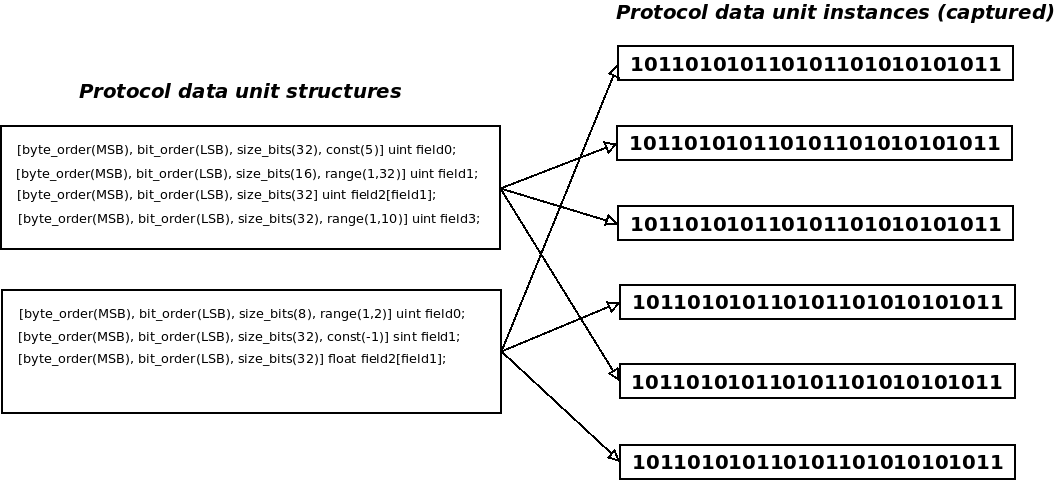
\includegraphics[width=0.8\textwidth]{net_proto_gen}
\end{center}
\caption{Network protocol genotype}
\label{fig:net_proto_gen}
\end{figure}

Well we're trying to figure out the structuring of protocol data units passed to the input.
Considering there can be more than one in a particular network protocol instance, 
the solution consists of a number of \emph{pdu structures}. Other than structuring, 
every pdu structure must have assigned an subset of input. This \emph{pdu structure-pdu instances} 
relation tells us which part of input is \emph{`described'} by which pdu structure.

The genotype consists (Figure \ref{fig:net_proto_gen}) of pdu structures and every
pdu structure is assigned a subset of pdu instances. A pdu structure is built of
\emph{fields}. A field can be of \emph{uint, sint and float} types pertaining to
unsigned and signed integers, and floating point numbers. Further more a field can
be a sized array which size can be set constant or set by other fields in the same
pdu structure.

Every field contains \emph{attributes} which describes its transfer syntax and semantics.
The defined attributes are:
\begin{description}
	\item[size\textunderscore{}bits] Size of the element in bit measure.
	\item[byte\textunderscore{}order] Byte ordering for a byte sized field.
	\item[bit\textunderscore{}order] Bit ordering.
	\item[range] Semantic attribute that defines a field value range.
	\item[const] Semantic attribute that defines a field is constant in value.
\end{description}

Our goal is to learn the type of fields in a pdu structure and their attributes.

The network protocol genotype is implemented within ECF framework in \emph{`NetProtoGen.cpp'}
file. It has registered parameters for setting the maximal pdu structures number
and of defining the number of captured data (pdu instances) to be considered a 
learning set:

\lstset{language=XML}
\lstset{basicstyle=\tiny}
\lstset{caption={Network protocol genotype parameters},label=lst:xml_netproto_gen}
\begin{lstlisting}[frame=tb]
<Genotype>
	<NetProto>
		<Entry key="max_pdus">4</Entry>
		<Entry key="num_cap_pdus">1000</Entry>
	</NetProto>
</Genotype>
\end{lstlisting}


\section{Genetic operators}
ECF provides all of the necessary core elements such as algorithm and fitness
components. Our job is to develop three operators for our newly defined network
protocol genotype. The first is the evaluation operator, then the crossover and
mutation operators.

\subsection{Evaluation}
This was probably the most challenging part to implement. It consists of generating
Lua code which performs the dissection of pdu instances according to a pdu structuring 
information held by the genotype. This code is invoked from the C++ environment
and executed in Lua environment. Other than parsing it calculates the fitness 
for that genotype instance.

The fitness calculation is based on semantic validity of fields with assigned
semantic attributes such as range, constant and array size semantic attributes.
Note that the pdu structure size can, in general, be determined in runtime, so
fitness calculation takes the size mismatch for every pair of pdu structure and 
pdu instance into consideration.

The constant and range attributes are checked for a field in a pdu structure and
for every pdu instance assigned to this pdu structure. Any violation of these
semantic restrictions is punished.

Two things can happen when parsing a field. First he field size can index data 
beyond a pdu instance size. Such occurrence must be punished by the evaluator.
The second thing can indicate a valid data space inside the size boundaries of
a pdu instance. This situation must be rewarded by the evaluator.

When the parsing of a single pdu instance is done according to structuring rules
of a pdu structure, the size mismatch is calculated and punished by the evaluator.

The evaluation operator is implemented in \emph{`NetProtoEvalOp.cpp'}. Its registered
parameter sets the file name of the input file which contains the pdu instances.

\subsection{Crossover}
Crossover is a genetic operator used to combine genetic material of \emph{parents}
to produce a new individual, a \emph{child}. A crossover operation represents a
directed search component of genetic algorithms, oppose to a mutation operation 
which represents a random search component. By performing a crossover operation 
on two individuals we hope to explore the solution space near them, hopefully 
finding a better solution.

There are two step in recombining network protocol genotypes. The first takes
two random pdu structures from both parents, and performs a sort of one cross-point
crossover with points represented as fields. The second operation deals with
pdu instance assignments. If a genotype has the same number of pdu structures
then the pdu instance assignments are copied to a child from randomly chosen 
parent.

Crossover is implemented in \emph{`NetProtoCrxOp.cpp'} and it has no registered
parameters.

\subsection{Mutation}
This is the simplest operation, and you can get pretty creative when designing 
a mutation operation. A network protocol genotype mutation operator also operates 
in two phases. The first randomly chooses a pdu structure and rebuilds it from 
scratch and the second resets the pdu instance assignments.

Mutation is implemented in \emph{`NetProtoMutOp.cpp'} and it has no registered
parameters.

\chapter{Conclusion}
Time invested in designing and developing the \emph{Wire} language for network
protocol specification resulted in clear definitions of language purpose, lexical
conventions, syntax and semantics. A cross-platform serialization engine has been
developed (and ported to Lua) in C on which the generated code is heavily dependent. A priority is the 
implementation of a Wire communication engine, or integration with existing open-source 
solutions. Future works consists of making a Python based code generation plug-in 
architecture, for more practical and easier code generation. Furthermore the 
GNU M4 macro language is to be utilized for implementation of Wire code inclusions.

The proposition that the task of automatic network protocol data units recognition
can be solved using the genetic algorithms has proven faulty. Even in theoretical
considerations the choice of using meta-heuristic search methods is wrong. The reason 
being that protocol data unit fields are, most commonly, mutually independent and lack the semantic
relationships. Therefore the genetic evaluator has no way, or little way, of determining
a fitness of an individual. Nevertheless a network protocol genotype has been developed
using the C++ ECF framework, including the genetic operators (evaluator, crossover, mutation).
The test example included `recognition' of \emph{Internet Protocol} (IP) data units. 


\begin{abstract}
Thesis gives an overview on network protocol theory including protocol design, 
specification and implementation. A network protocol specification language called
Wire has been developed in the scope of this thesis. Detailed descriptions on
the analysis of the Wire language are given, as well as on code generation. An
overview of Wire language is provided using an example network protocol.

The problem of automatic network protocol recognition has been addressed in the scope
of this thesis. Genetic algorithms have been utilized for solving this problem, 
therefore a network protocol genotype and corresponding genetic operators have been
developed and implemented using the C++ Evolutionary Computation Framework.

\keywords{network protocol theory, abstract syntax notation, 
wire definition language, automatic recognition, genetic algorithms, 
evolutionary computation framework}
\end{abstract}

\title{Metode predstavljanja i automatskog prepoznavanja mrežnih protokola}
\begin{sazetak}
Rad daje pregled na teorijom mrežnih protokola, uključujući dizajn, specifikaciju
i implementaciju mrežnih protokola. U sklopu rada ostvaren je jezik za specifikaciju 
mrežnih protokola nazvan Wire. Analiza jezika Wire i stvaranje koda su detaljno objašnjeni.
Napravljen je pregled nad jezikom Wire koristeći primjerni mrežni protokol.

Problem automatskog prepoznavanja mrežnih protokola također se obrađuje u sklopu
ovog rada. Za rješavanje tog problema korišteni su genetski algoritmi, stoga su
razvijeni genotip za predstavljanje mrežnog protokola i odgovarajući genetski operatori
koristeći C++ okruženje Evolutionary Computation Framework.

\kljucnerijeci{teorija mrežnih protokola, notacija za apstraktnu sintaksu, wire jezik, 
automatsko prepoznavanje, genetski algoritmi, evolutionary computation framework}
\end{sazetak}

\bibliography{diplomski}
\bibliographystyle{fer}

\appendix
\chapter{Wire lexical definitions}
\lstset{language=C}
\lstset{basicstyle=\tiny}
\lstset{caption={wire.l},label=lst:wire_l}
\lstset{numbers=left, numberstyle=\tiny, stepnumber=1, numbersep=5pt}
\lstinputlisting{../../wire.l}

\chapter{Wire syntax definitions}
\lstset{language=C}
\lstset{basicstyle=\tiny}
\lstset{caption={Wire BNF grammar listing produced by GNU Bison report mechanism},label=lst:wire_syn_bnf}
\lstset{numbers=left, numberstyle=\tiny, stepnumber=1, numbersep=5pt}
\lstinputlisting{wire_syn_bnf.report}

\end{document}
